
\chapter{Analyse et spécification des besoins}
\label{chap:Analyse et spécification des besoins}

Ce chapitre présente l'analyse de l'existant et la spécification des besoins pour l'intégration de Payconiq by Bancontact. Il examine les méthodes de paiement actuelles, les spécificités du marché belge, le processus de paiement en place, ainsi que les besoins fonctionnels et non fonctionnels.
\pagebreak

\section{Étude de l’existant}
\subsection{Méthodes de paiement actuelles}
Le site e-commerce de la marque propose actuellement une gamme diversifiée de méthodes de paiement reconnues mondialement, comprenant :
\begin{itemize}
    \item Visa
    \item MasterCard
    \item PayPal
    \item Klarna Pay Now
    \item Klarna Pay Later
    \item Chanel Gift Card
\end{itemize}
Bien que ces options répondent efficacement aux besoins d'une clientèle internationale, elles ne tiennent pas compte des spécificités locales de certains marchés clés, en particulier celui de la Belgique.
\subsection{Particularités du marché belge}
En Belgique, Bancontact s'est imposé comme l'une des méthodes de paiement privilégiées. Initialement conçu comme un système de paiement par carte de débit nationale, Bancontact est devenu un élément incontournable du paysage financier belge. Cette solution offre aux consommateurs la possibilité d'effectuer des paiements directs depuis leur compte bancaire, que ce soit en magasin, en ligne ou via une application mobile.
Face à l'évolution rapide des technologies et des attentes des consommateurs, Bancontact a réalisé une fusion stratégique avec Payconiq, une solution de paiement mobile innovante. Cette alliance a donné naissance à Payconiq by Bancontact , offrant aux utilisateurs belges une solution de paiement intégrée couvrant à la fois les transactions par carte et les paiements mobiles via une application dédiée.
L'adoption massive de cette solution en Belgique en fait un élément incontournable pour tout e-commerce aspirant à s'implanter solidement sur ce marché. Les chiffres parlent d'eux-mêmes : en 2023, près de 2 millions de Belges \cite{Belge} ont utilisé Payconiq pour leurs paiements mobiles, soulignant l'importance cruciale de cette méthode dans l'écosystème des paiements locaux.
\subsection{Justification de l'intégration de Payconiq by Bancontact }
L'intégration de Payconiq by Bancontact  sur notre plateforme e-commerce présente plusieurs avantages stratégiques, particulièrement pour conquérir et fidéliser la clientèle belge \cite{Payconic}:
\begin{itemize}
    \item [$\bullet$]\textbf{Adoption généralisée :} Avec une base d'environ 2 millions d'utilisateurs Payconiq et une forte pénétration de Bancontact dans les habitudes de paiement quotidiennes, cette solution est profondément ancrée dans le comportement des consommateurs belges.
    \item [$\bullet$]\textbf{Simplicité et ergonomie :} L'application "Payconiq by Bancontact" offre une expérience de paiement fluide et intuitive, reposant sur un simple scan de QR code, ce qui optimise considérablement le parcours client.
    \item [$\bullet$]\textbf{Sécurité renforcée :} La synergie entre les systèmes Bancontact et Payconiq garantit un niveau
    de sécurité optimal pour les transactions, s’appuyant sur des protocoles de sécurité robustes et éprouvés comme le cryptage de bout en bout pour protéger les données sensibles. Ils utilisent aussi une couche supplémentaire de protection via l'authentification forte du client (SCA) conformément aux normes européennes PSD2. Cette authentification multiple peut inclure des facteurs biométriques, des mots de passe ou des codes à usage unique, minimisant ainsi les risques de fraude.
    \item [$\bullet$]\textbf{Interopérabilité bancaire :} Le support étendu de Payconiq par les principales institutions bancaires belges facilite son adoption et renforce la commodité pour les clients, en centralisant leurs opérations financières.
    \item [$\bullet$]\textbf{Essor des paiements mobiles :} Face à la croissance exponentielle des paiements mobiles en Belgique, l'intégration de solutions comme Payconiq s'avère cruciale pour capter et fidéliser une clientèle, particulièrement auprès des jeunes générations habituées aux transactions via smartphone.
\end{itemize}
\subsection{Processus de paiement actuel}
Le processus de paiement en place, présenté dans la figure \ref{fig:processus}, repose sur l'interaction harmonieuse de plusieurs systèmes interdépendants, chacun jouant un rôle déterminant dans la sécurisation des transactions et l'optimisation du traitement des commandes. 
\begin{center}
    \centering
    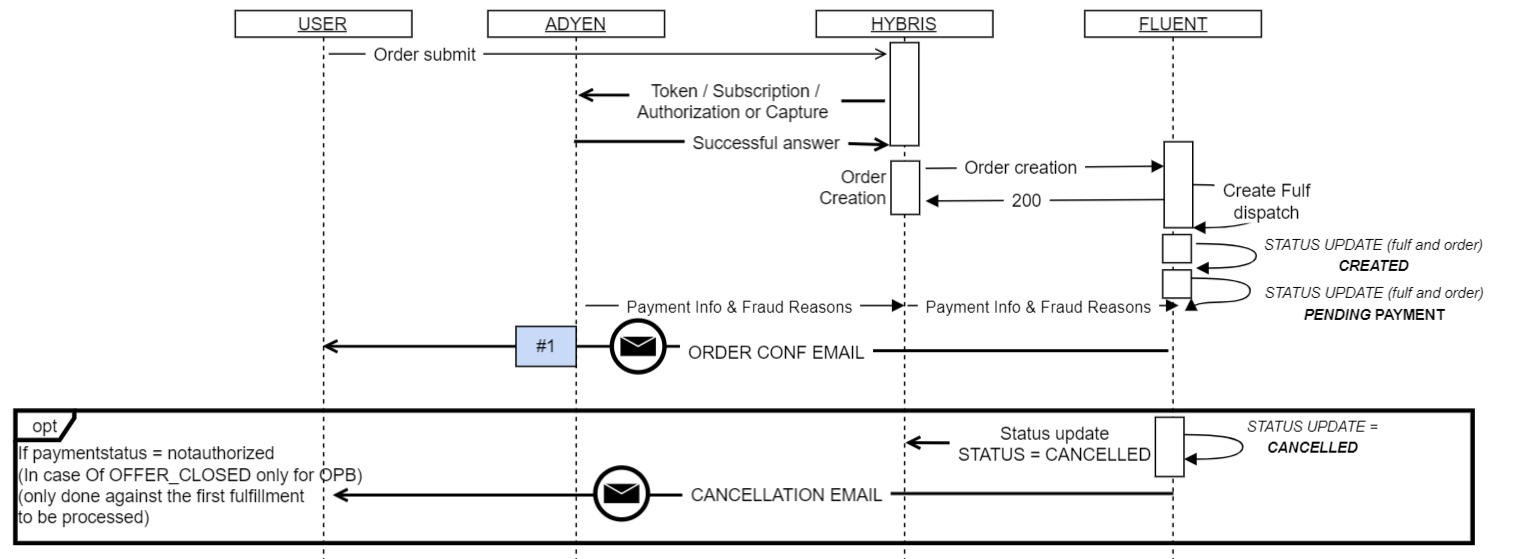
\includegraphics[width=19cm]{Figures/processus.jpeg}
    \captionof{figure}{Processus du paiement}
    \label{fig:processus}
\end{center}
Les composants clés du système sont les suivants :
\begin{itemize}
    \item [$\bullet$]\textbf{Hybris :} Plateforme e-commerce centrale, Hybris est responsable de la création des commandes une fois le paiement validé. Après la soumission d'une commande par l'utilisateur, Hybris communique avec Adyen pour le traitement du paiement. Une fois la confirmation reçue, Hybris crée officiellement la commande et notifie Fluent pour la gestion de l'expédition et du suivi.
    \item [$\bullet$]\textbf{Adyen :} En tant que fournisseur de services de paiement, Adyen gère la transaction financière. Il traite les détails du paiement transmis par Hybris, réalisant des actions telles que l'autorisation, la capture des fonds, ou la gestion des abonnements. Adyen joue un rôle clé dans la sécurisation et la validation des paiements avant la finalisation de la commande.
    \item [$\bullet$]\textbf{Fluent :} Système de gestion logistique, Fluent est responsable du cycle de vie de la commande après sa création dans Hybris. Il assure le suivi du processus de traitement, y compris la préparation de l'expédition, et met à jour les statuts de la commande (par exemple, "CREATED", "PENDING PAYMENT", "CANCELLED"). Fluent communique également avec Hybris pour informer les utilisateurs de l'état de leur commande.
\end{itemize}
Pour mieux comprendre le fonctionnement de ces composants, examinons le flux du processus de paiement étape par étape :
\begin{enumerate}
    \item \textbf{Initiation :} Le client valide son panier et soumet sa commande.
    \item \textbf{Transmission :} Hybris envoie une requête à Adyen pour déclencher le processus de paiement.
    \item \textbf{Traitement :} Adyen exécute la transaction et renvoie une confirmation à Hybris.
    \item \textbf{Création :} Hybris enregistre la commande et notifie Fluent pour la gestion logistique.
    \item \textbf{Suivi :} Fluent assure la gestion des statuts de commande et informe Hybris pour la mise à jour du client.
\end{enumerate}
\section{Identification et analyse des exigences}
Dans le cadre de l'intégration de Payconiq à la plateforme e-commerce du client, il est essentiel de définir clairement les besoins fonctionnels et non fonctionnels du projet. 
Cette étude permettra d'identifier les exigences spécifiques liées à cette intégration, assurant ainsi une mise en œuvre réussie et une expérience utilisateur optimale. 

\subsection{Exigences fonctionnelles}

\subsubsection{Identification des fonctionnalités}
\begin{itemize}
    \item [$\bullet$]\textbf{Sélection de Payconiq comme méthode de paiement :} L’option Payconiq devra être disponible lors de la finalisation de la commande, présentée de manière intuitive et clairement distinguée parmi les autres choix de paiement.
    \item [$\bullet$]\textbf{Génération et affichage du QR Code pour le paiement :} Lors de la confirmation de la commande avec Payconiq, un QR code unique devra être généré automatiquement et affiché à l’utilisateur pour permettre un paiement sécurisé via l’application Payconiq.
    \item [$\bullet$]\textbf{Suivi des transactions dans l'historique des commandes :} Les transactions effectuées avec Payconiq devront être accessibles dans l’historique des commandes de l’utilisateur, avec une identification claire comprenant la date, le montant et l’état du paiement.
    \item [$\bullet$]\textbf{Envoi d'un email de confirmation de commande :} Après la finalisation de la commande, un email de confirmation devra être envoyé à l’utilisateur, incluant les détails de la commande, la méthode de paiement utilisée (Payconiq), le montant total et les informations de suivi de la commande.
    \item [$\bullet$]\textbf{Message d'erreur en cas d'échec du paiement :} En cas d’échec du paiement avec Payconiq, un message d’erreur explicite devra informer l’utilisateur du problème, avec des options de paiement alternatives proposées pour finaliser la transaction sans interruption.
\end{itemize}

\subsubsection{Diagramme de cas d’utilisation}
\begin{center}
    \centering
    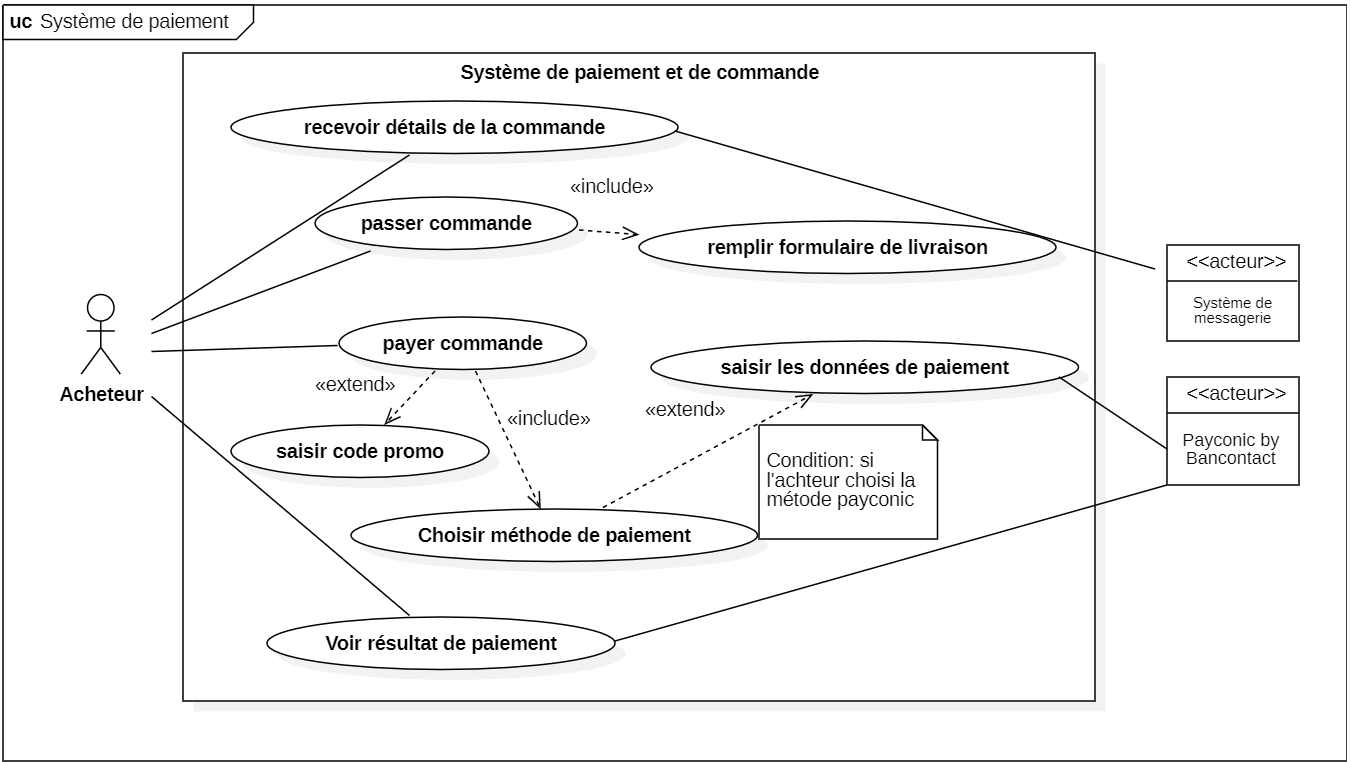
\includegraphics[width=19cm]{Figures/usecase.png}
    \captionof{figure}{Diagramme de cas d'utilisation}
    \label{fig:usecase}
\end{center}

\subsubsection{Analyse des cas d'utilisation}
\begin{longtable}{|p{4cm}|p{11cm}|}
\hline
\multicolumn{2}{|c|}{\textbf{Passer Commande}} \\ \hline
\textbf{But} & Confirmer l'achat des produits ajoutés au panier \\ \hline
\textbf{Acteur} & Acheteur \\ \hline
\textbf{Pré-conditions} & Avoir des produits dans le panier \\ \hline
\textbf{Post-conditions} & Saisir les informations de paiement \\ \hline
\textbf{Scénario normal} &
\begin{itemize}
    \item Consulter le panier;
    \item Cliquer sur "Passer commande";
    \item Choisir le mode de livraison (à domicile ou click and collect);
    \item Saisir les informations de livraison;
    \item Saisir l'adresse de facturation (peut être différente de l'adresse de livraison);
    \item Vérification les informations requises;
    \item Redirection vers la page de paiement.
\end{itemize} \\ \hline
\textbf{Scénario alternatif} &
\begin{enumerate}
    \item Un produit sélectionné n'est plus disponible en stock
    \begin{itemize}
        \item Affichage du message "Produit indisponible"
    \end{itemize}
    \item Manque d'informations requises
    \begin{itemize}
        \item Affichage du message indiquant l'information manquante
    \end{itemize}
\end{enumerate} \\ \hline
\caption{Description textuelle du cas d'utilisation "Passer Commande"}
\label{tab:passer_commande}
\end{longtable}

\begin{longtable}{|p{4cm}|p{11cm}|}
    \hline
    \multicolumn{2}{|c|}{\textbf{Finaliser l'achat d'une commande}} \\ \hline
    \textbf{But} & Finaliser l'achat d'une commande \\ \hline
    \textbf{Acteur} & Acheteur \\ \hline
    \textbf{Pré-conditions} & 
    \begin{itemize}
        \item Passer la commande
        \item Disposer d'un compte payconiq actif
    \end{itemize} \\ \hline
    \textbf{Post-conditions} & Saisir les informations de paiement \\ \hline
    \textbf{Scénario normal} &
    \begin{itemize}
        \item Sélectionner Payconiq comme méthode de paiement;
        \item Génération d'un QR code Payconiq;
        \item Ouvrir l'application Payconiq by Bancontact et scanner le QR code;
        \item Confirmer le montant et autoriser le paiement dans l'application;
        \item Redirection vers une page de confirmation de commande;
        \item Recevoir une confirmation de paiement sur le site et par e-mail.
    \end{itemize} \\ \hline
    \textbf{Scénario alternatif} &
    \begin{enumerate}
        \item Fonds insuffisants
        \begin{itemize}
            \item Affichage du message "Fonds insuffisants"
        \end{itemize}
        \item Manque d'informations requises
        \begin{itemize}
            \item Affichage du message indiquant l'information manquante
        \end{itemize}
    \end{enumerate} \\ \hline
    \caption{Description textuelle du cas d'utilisation "Finaliser l'achat d'une commande"}
    \label{tab:finaliser_commande}
    \end{longtable}


\subsection{Exigences non-fonctionnelles}

Les exigences non-fonctionnelles sont essentielles pour assurer la qualité des services de la plateforme, notamment en termes de sécurité, de maintenabilité et de disponibilité. Elles garantissent non seulement une expérience utilisateur optimale, mais aussi la pérennité et l'efficacité du système face aux évolutions technologiques et aux besoins des utilisateurs. Parmi ces exigences, on peut citer :

\begin{itemize}
    \item [$\bullet$]\textbf{Sécurité :} La protection des informations sensibles des utilisateurs est cruciale dans tout système de paiement en ligne. L'intégration de Payconiq requiert une attention particulière à ces aspects pour éviter tout accès non autorisé et toute manipulation malveillante des données.
    \item [$\bullet$]\textbf{Maintenabilité :} La maintenabilité du système est essentielle pour garantir sa longévité et sa capacité à évoluer. Un code clair, bien structuré, et conforme aux meilleures pratiques de développement facilite l'ajout de nouvelles fonctionnalités et permet une correction rapide des bugs. Une bonne maintenabilité permet aux équipes de développement de diagnostiquer et de résoudre efficacement les problèmes, de déployer des mises à jour sans perturber le fonctionnement du système, et d'adapter rapidement le système aux évolutions technologiques et aux besoins des utilisateurs.
    \item [$\bullet$]\textbf{Disponibilité :} Le système doit être conçu pour faciliter le diagnostic, la résolution des problèmes, le déploiement des mises à jour, et l’adaptation aux évolutions technologiques et aux besoins des utilisateurs.
\end{itemize}


\section*{Conclusion}
La phase d'analyse de l'existant et de spécification des besoins est cruciale pour le succès de notre projet. Nous avons abordé cette phase en examinant le processus actuel et en identifiant les cas d'utilisation spécifiques au marché belge. Nous avons ensuite entamé l'analyse des besoins fonctionnels et non fonctionnels. Dans le chapitre suivant, nous aborderons la conception détaillée du projet.